\chapter{UML Models} \label{chap5}

\section{Use Case Diagram}
The Figure \ref{fig:usecase} gives an overview on the main actors involved in the system and the functionalities that they are able to execute.

\begin{figure}[htbp]
\centering
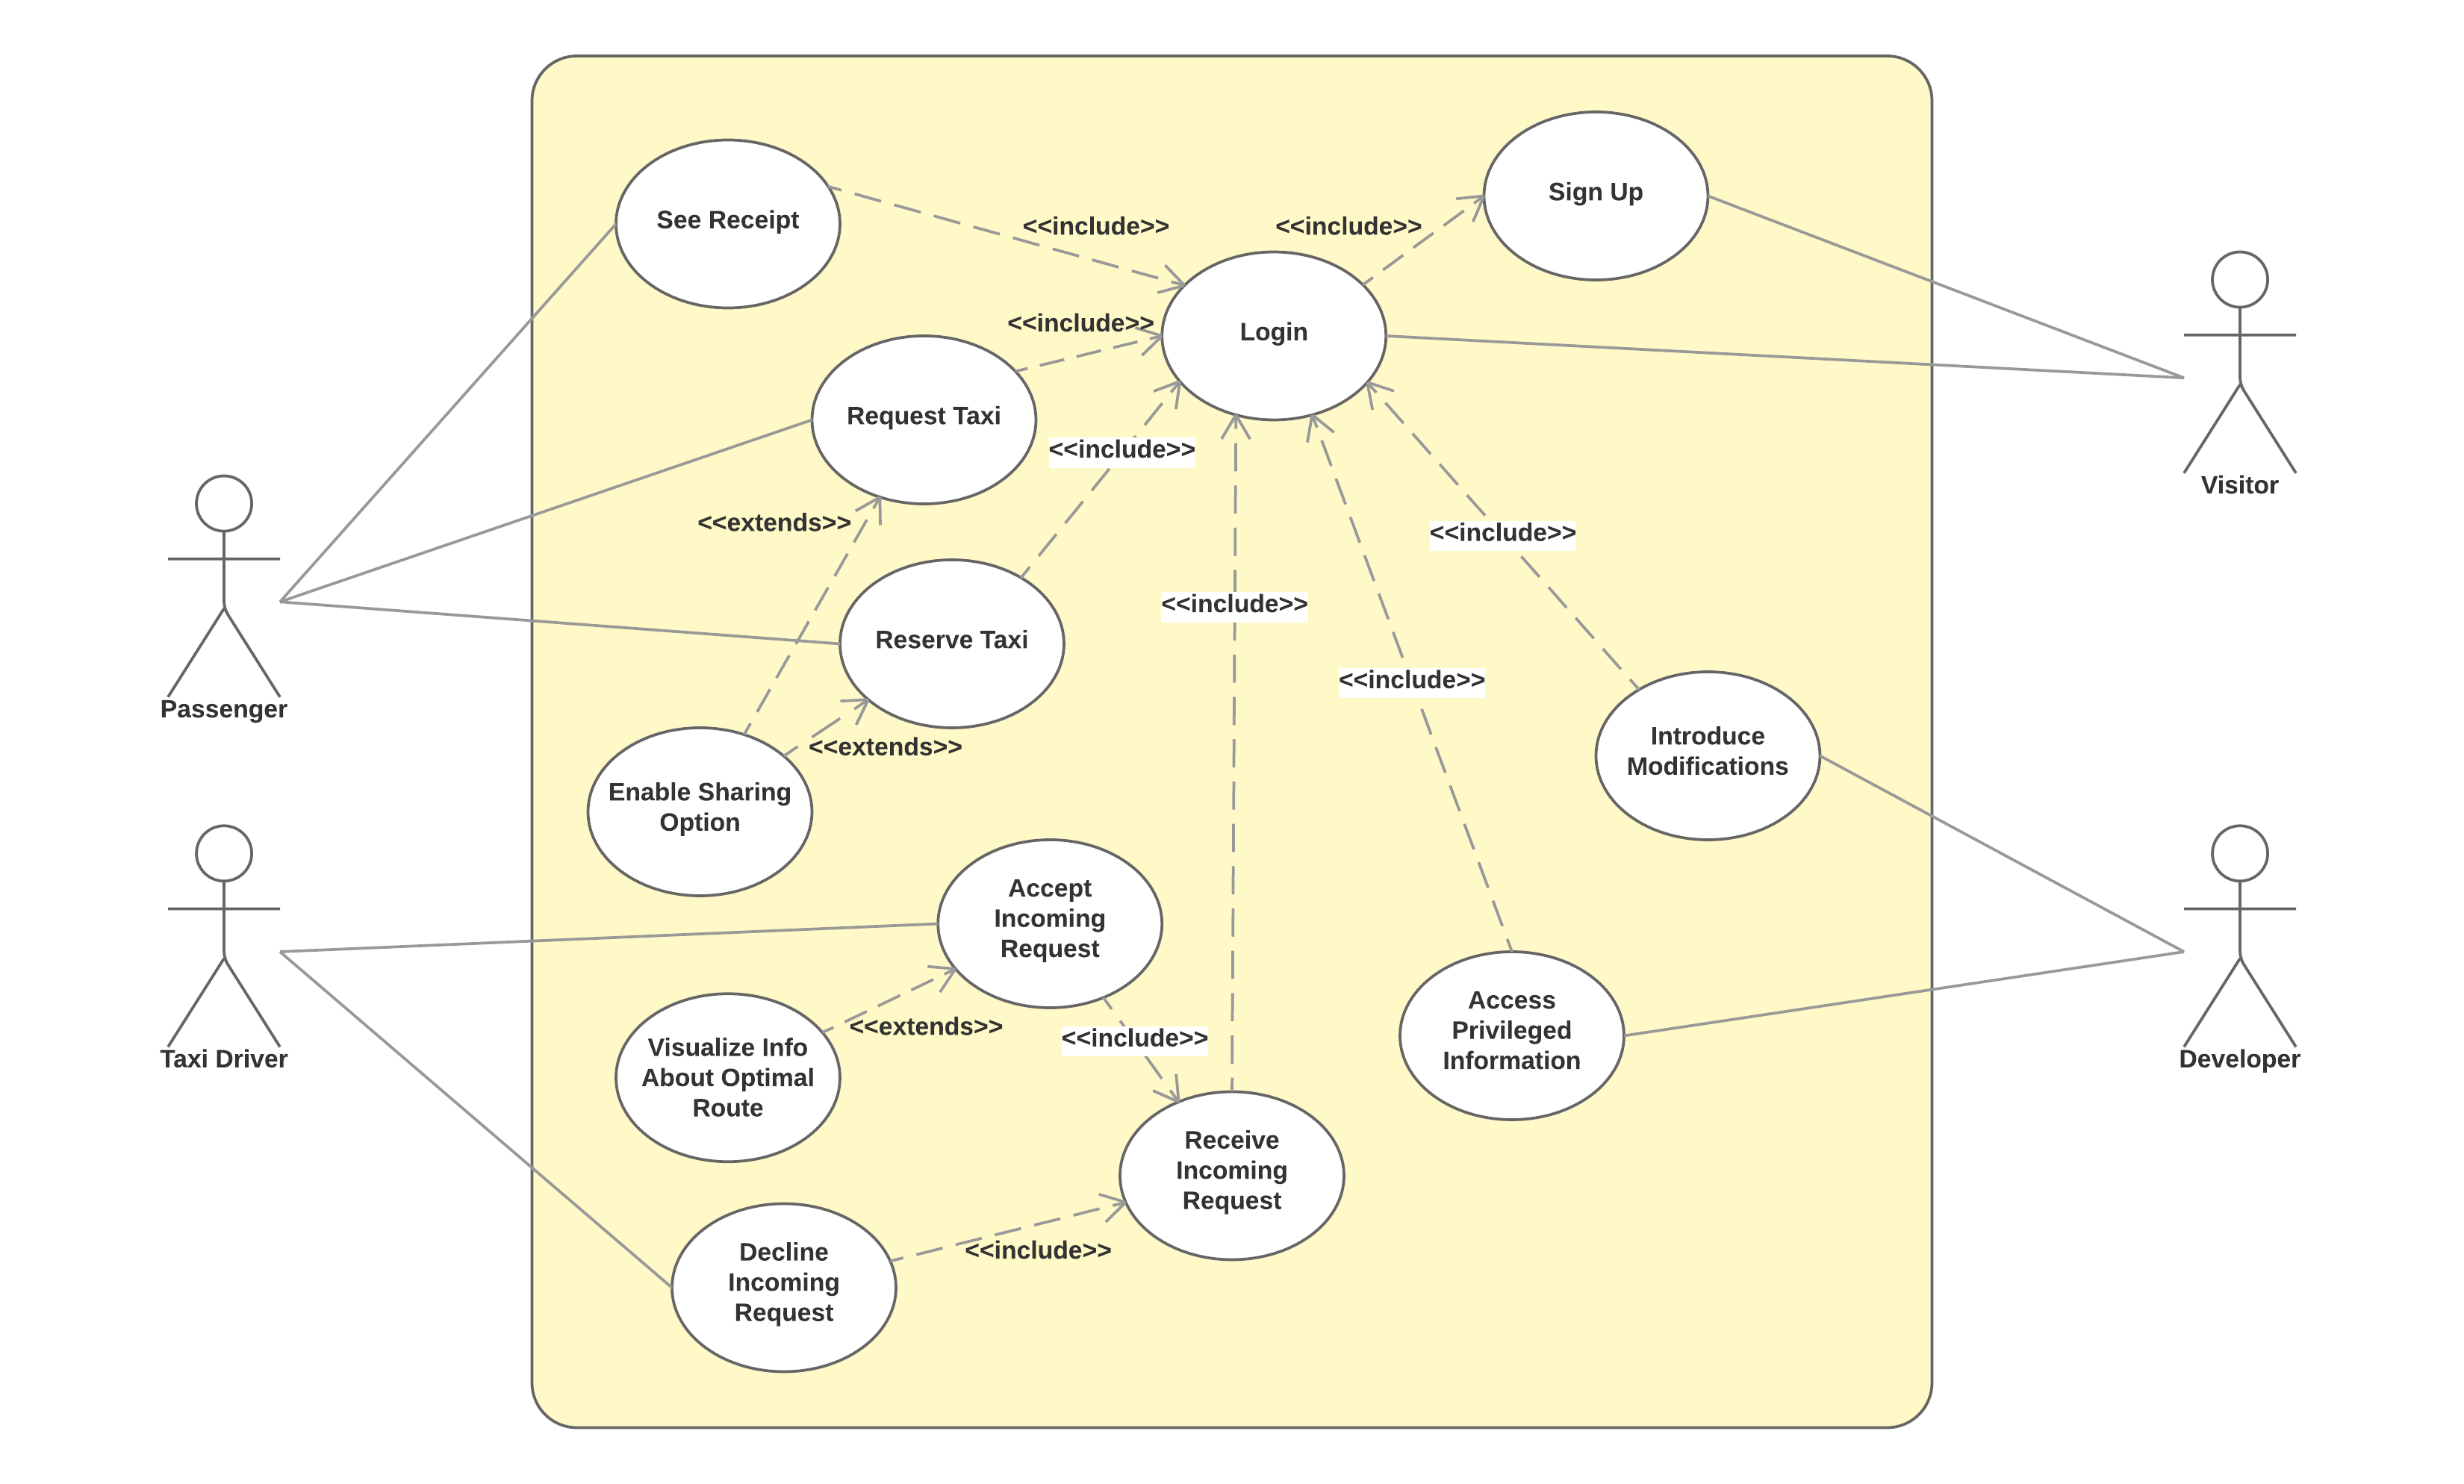
\includegraphics[width=\textwidth]{cpt/img/UseCase}
\caption{Use Case Diagram}
\label{fig:usecase}
\end{figure}

\section{Use Case Descriptions}

\subsubsection{Sign Up}

\begin{table}[htbp]
\begin{center}
\begin{tabular}[t]{p{0.35\textwidth}p{0.65\textwidth}}

\hline
Actor & Visitor \\
\hline
Related Requirements & [R01], [R02] \\
\hline
Goal in context & [G01] \\
\hline
Precondition & the Visitor access the initial application interface \\
\hline
Successful end condition & the Visitor is registered on the system as a passenger, taxi driver or developer \\
\hline
Failed end condition & the Visitor is not able to register. He/She is asked to try again \\
\hline
Trigger & the Visitor selects the ''Sign up'' button \\
\hline
Main Flow & \textbf{1.} the Visitor fills in the registration form with his/her personal data \\
& \textbf{2.} the Visitor selects what kind of user he/she is \\
& \textbf{3.} the Visitor submits the form \\
& \textbf{4.} the System saves the new account information in its database \\
& \textbf{5.} the Visitor receives a confirmation message\\
\hline
Extensions & --- \\
\hline

\end{tabular}
\end{center}
\caption{Sign Up Use Case}
\end{table}
\clearpage

\subsubsection{Login}

\begin{table}[htbp]
\begin{center}
\begin{tabular}[t]{p{0.35\textwidth}p{0.65\textwidth}}

\hline
Actor & Visitor \\
\hline
Related Requirements & [R03], [R04] \\
\hline
Goal in context & [G02] \\
\hline
Precondition & the Visitor access the initial application interface \\
\hline
Successful end condition & 
the Visitor can now access his/her profile and interact with the system according to his/her privileges
 \\
\hline
Failed end condition & the Visitor is not able to login. He/She is asked to try again \\
\hline
Trigger & the Visitor selects the ''Log In'' button \\
\hline
Main Flow & \textbf{1.} the Visitor insert username and password \\
& \textbf{2.}the System verifies his/her credentials \\
& \textbf{3.} the Visitor receives a confirmation message \\
\hline
Extensions & --- \\
\hline

\end{tabular}
\end{center}
\caption{Log In Use Case}
\end{table}
\clearpage

\subsubsection{Request Taxi}

\begin{table}[htbp]
\begin{center}
\begin{tabular}[t]{p{0.35\textwidth}p{0.65\textwidth}}

\hline
Actor & Passenger \\
\hline
Related Requirements & [R05], [R06], [R07], [R08], [R09], [R10], [R11] \\
\hline
Goal in context & [G03], [G05] \\
\hline
Precondition & the Passenger must be logged in \\
\hline
Successful end condition & 
the Passenger can access an information page with confirmation, taxi code and waiting time
 \\
\hline
Failed end condition & the Passenger receives an error message  \\
\hline
Trigger & the Passenger select the ''Request'' button to access the request interface \\
\hline
Main Flow & \textbf{1.} the System sets the current position of the Passenger as the origin for the ride \\
& \textbf{2.} the Passenger insert the destination of the ride \\
& \textbf{3.} the Passenger submits the request to the System \\
& \textbf{4.} the Passenger receives a confirmation message \\
\hline
Extensions & \textbf{3.1} the Passenger selects the ''enable sharing'' option \\
\hline

\end{tabular}
\end{center}
\caption{Request Taxi Use Case}
\end{table}
\clearpage

\subsubsection{Reserve Taxi}

\begin{table}[htbp]
\begin{center}
\begin{tabular}[t]{p{0.35\textwidth}p{0.65\textwidth}}

\hline
Actor & Passenger \\
\hline
Related Requirements & [R05], [R06], [R07], [R08], [R09] \\
\hline
Goal in context & [G04] \\
\hline
Precondition & the Passenger must be logged in \\
\hline
Successful end condition & 
the Passenger can access an information page with confirmation, taxi code and summary of the reservation
 \\
\hline
Failed end condition & the Passenger receives an error message  \\
\hline
Trigger & the Passenger select the ''Reserve'' button to access the reservation interface \\
\hline
Main Flow & \textbf{1.} the Passenger insert origin and destination for the ride \\
& \textbf{2.} the Passenger insert the reservation time \\
& \textbf{3.} the Passenger submits the reservation to the System \\
& \textbf{4.} the Passenger receives a confirmation message \\
\hline
Extensions & \textbf{3.1} the Passenger selects the ''enable sharing'' option \\
\hline

\end{tabular}
\end{center}
\caption{Reserve Taxi Use Case}
\end{table}
\clearpage

\subsubsection{Enable Sharing Option}

\begin{table}[htbp]
\begin{center}
\begin{tabular}[t]{p{0.35\textwidth}p{0.65\textwidth}}

\hline
Actor & Passenger \\
\hline
Related Requirements & [R12], [R13], [R14], [R15] \\
\hline
Goal in context & [G06] \\
\hline
Precondition & the Passenger must be logged in \\
\hline
Successful end condition & 
the Passenger can share the ride with other passengers \\
\hline
Failed end condition & there are no other passengers willing to share the ride  \\
\hline
Trigger & the Passenger selects the ''enable sharing'' option from the request or the reservation interface \\
\hline
Main Flow & \textbf{1.} the System verifies whether there are other passengers willing to share the ride \\
& \textbf{2.} the System calculate the fee percentage for the ride \\
& \textbf{3.} the Passenger receives a message with information about the shared ride \\
\hline
Extensions & --- \\
\hline

\end{tabular}
\end{center}
\caption{Enable Sharing Option Taxi Use Case}
\end{table}
\clearpage

\subsubsection{See Receipt}

\begin{table}[htbp]
\begin{center}
\begin{tabular}[t]{p{0.35\textwidth}p{0.65\textwidth}}

\hline
Actor & Passenger \\
\hline
Related Requirements & [R16] \\
\hline
Goal in context & [G07] \\
\hline
Precondition & the Passenger has completed the ride \\
\hline
Successful end condition & the Passenger access the receipt of the last ride \\
\hline
Failed end condition & the Passenger receives an error message  \\
\hline
Trigger & the Passenger select the ''All Receipts'' button \\
\hline
Main Flow & \textbf{1.} the Passenger access the chronology of his/her rides \\
& \textbf{2.} the Passenger selects the last ride \\
& \textbf{3.} the Passenger sees the receipt for the ride \\
\hline
Extensions & \textbf{3.1} the Passenger saves the receipt on his/her device \\
& \textbf{3.2} the Passenger prints the receipt \\
\hline

\end{tabular}
\end{center}
\caption{See Receipt Use Case}
\end{table}
\clearpage

\subsubsection{Accept Incoming Requests}

\begin{table}[htbp]
\begin{center}
\begin{tabular}[t]{p{0.35\textwidth}p{0.65\textwidth}}

\hline
Actor & Taxi Driver \\
\hline
Related Requirements & [R17] \\
\hline
Goal in context & [G10] \\
\hline
Precondition & the Taxi Driver has received an incoming request or reservation \\
\hline
Successful end condition & the Taxi Driver accepts the request or reservation \\
\hline
Failed end condition & a System error occurs. An error message is shown to the Taxi Driver  \\
\hline
Trigger & --- \\
\hline
Main Flow & \textbf{1.} the System shows to the Taxi Driver a request or reservation coming from a Passenger \\
& \textbf{2.} the Taxi Driver clicks on the ''Accept'' button \\
\hline
Extensions & --- \\
\hline

\end{tabular}
\end{center}
\caption{Accept Incoming Requests Use Case}
\end{table}
\clearpage

\subsubsection{Decline Incoming Requests}

\begin{table}[htbp]
\begin{center}
\begin{tabular}[t]{p{0.35\textwidth}p{0.65\textwidth}}

\hline
Actor & Taxi Driver \\
\hline
Related Requirements & [R17] \\
\hline
Goal in context & [G10] \\
\hline
Precondition & the Taxi Driver has received an incoming request or reservation \\
\hline
Successful end condition & the Taxi Driver declines the request or reservation \\
\hline
Failed end condition & a System error occurs. An error message is shown to the Taxi Driver  \\
\hline
Trigger & --- \\
\hline
Main Flow & \textbf{1.} the System shows to the Taxi Driver a request or reservation coming from a Passenger \\
& \textbf{2.} the Taxi Driver clicks on the ''Decline'' button \\
\hline
Extensions & --- \\
\hline

\end{tabular}
\end{center}
\caption{Decline Incoming Requests Use Case}
\end{table}
\clearpage

\subsubsection{Receive Incoming Requests}

\begin{table}[htbp]
\begin{center}
\begin{tabular}[t]{p{0.35\textwidth}p{0.65\textwidth}}

\hline
Actor & Taxi Driver \\
\hline
Related Requirements & [R18] \\
\hline
Goal in context & [G09] \\
\hline
Precondition & the Taxi Driver must be logged in \\
\hline
Successful end condition & the Taxi Driver sees the request or reservation details and he/she is asked to click on ''Accept'' or ''Decline'' \\
\hline
Failed end condition & a System error occurs. An error message is shown to the Taxi Driver  \\
\hline
Trigger & the Passenger sends a request or reservation to the System \\
\hline
Main Flow & \textbf{1.} the System receives the reservation or request from a Passenger \\
& \textbf{2.} the Taxi Driver receives the reservation or request from the System \\
\hline
Extensions & --- \\
\hline

\end{tabular}
\end{center}
\caption{Receive Incoming Requests Use Case}
\end{table}
\clearpage

\subsubsection{Visualize Information About Optimal Route}

\begin{table}[htbp]
\begin{center}
\begin{tabular}[t]{p{0.35\textwidth}p{0.65\textwidth}}

\hline
Actor & Taxi Driver \\
\hline
Related Requirements & [R19], [R20] \\
\hline
Goal in context & [G11] \\
\hline
Precondition & --- \\
\hline
Successful end condition & the Taxi Driver sees the information about the optimal route for the booked ride \\
\hline
Failed end condition & a System error occurs. An error message is shown to the Taxi Driver  \\
\hline
Trigger & the Taxi Driver accept a request or reservation \\
\hline
Main Flow & \textbf{1.} the System calculates the optimal route for the accepted ride \\
& \textbf{2.} an information message is shown to the Taxi Driver \\
\hline
Extensions & --- \\
\hline

\end{tabular}
\end{center}
\caption{Visualize Information About Optimal Route Use Case}
\end{table}
\clearpage

\subsubsection{Introduce Modifications}

\begin{table}[htbp]
\begin{center}
\begin{tabular}[t]{p{0.35\textwidth}p{0.65\textwidth}}

\hline
Actor & Developer \\
\hline
Related Requirements & [R21] \\
\hline
Goal in context & [G12] \\
\hline
Precondition & the Developer must be logged in \\
\hline
Successful end condition & the Developer successfully introduces modification to the System \\
\hline
Failed end condition & a System error occurs. An error message is shown to the Developer  \\
\hline
Trigger & --- \\
\hline
Main Flow & \textbf{1.} the Developer access the ''Modification'' interface \\
& \textbf{2.} the Developer introduces modifications \\
& \textbf{3.} the Developer submits his/her modifications \\
\hline
Extensions & --- \\
\hline

\end{tabular}
\end{center}
\caption{Introduce Modifications Use Case}
\end{table}
\clearpage

\subsubsection{Access Privileged Information}

\begin{table}[htbp]
\begin{center}
\begin{tabular}[t]{p{0.35\textwidth}p{0.65\textwidth}}

\hline
Actor & Developer \\
\hline
Related Requirements & [R21] \\
\hline
Goal in context & [G12] \\
\hline
Precondition & the Developer must be logged in \\
\hline
Successful end condition & the Developer sees the information the he/she needs \\
\hline
Failed end condition & a System error occurs. An error message is shown to the Developer  \\
\hline
Trigger & --- \\
\hline
Main Flow & \textbf{1.} the Developer access the ''Information'' interface \\
& \textbf{2.} the Developer sees all the information about the System \\
\hline
Extensions & --- \\
\hline

\end{tabular}
\end{center}
\caption{Introduce Modifications Use Case}
\end{table}
\clearpage

\section{Class Diagram}
Here is presented the UML class diagram in Figure \ref{fig:classdiag}. This diagram will be updated during the developing process especially by adding all methods:

\begin{landscape}
\begin{figure}[h]
\centering
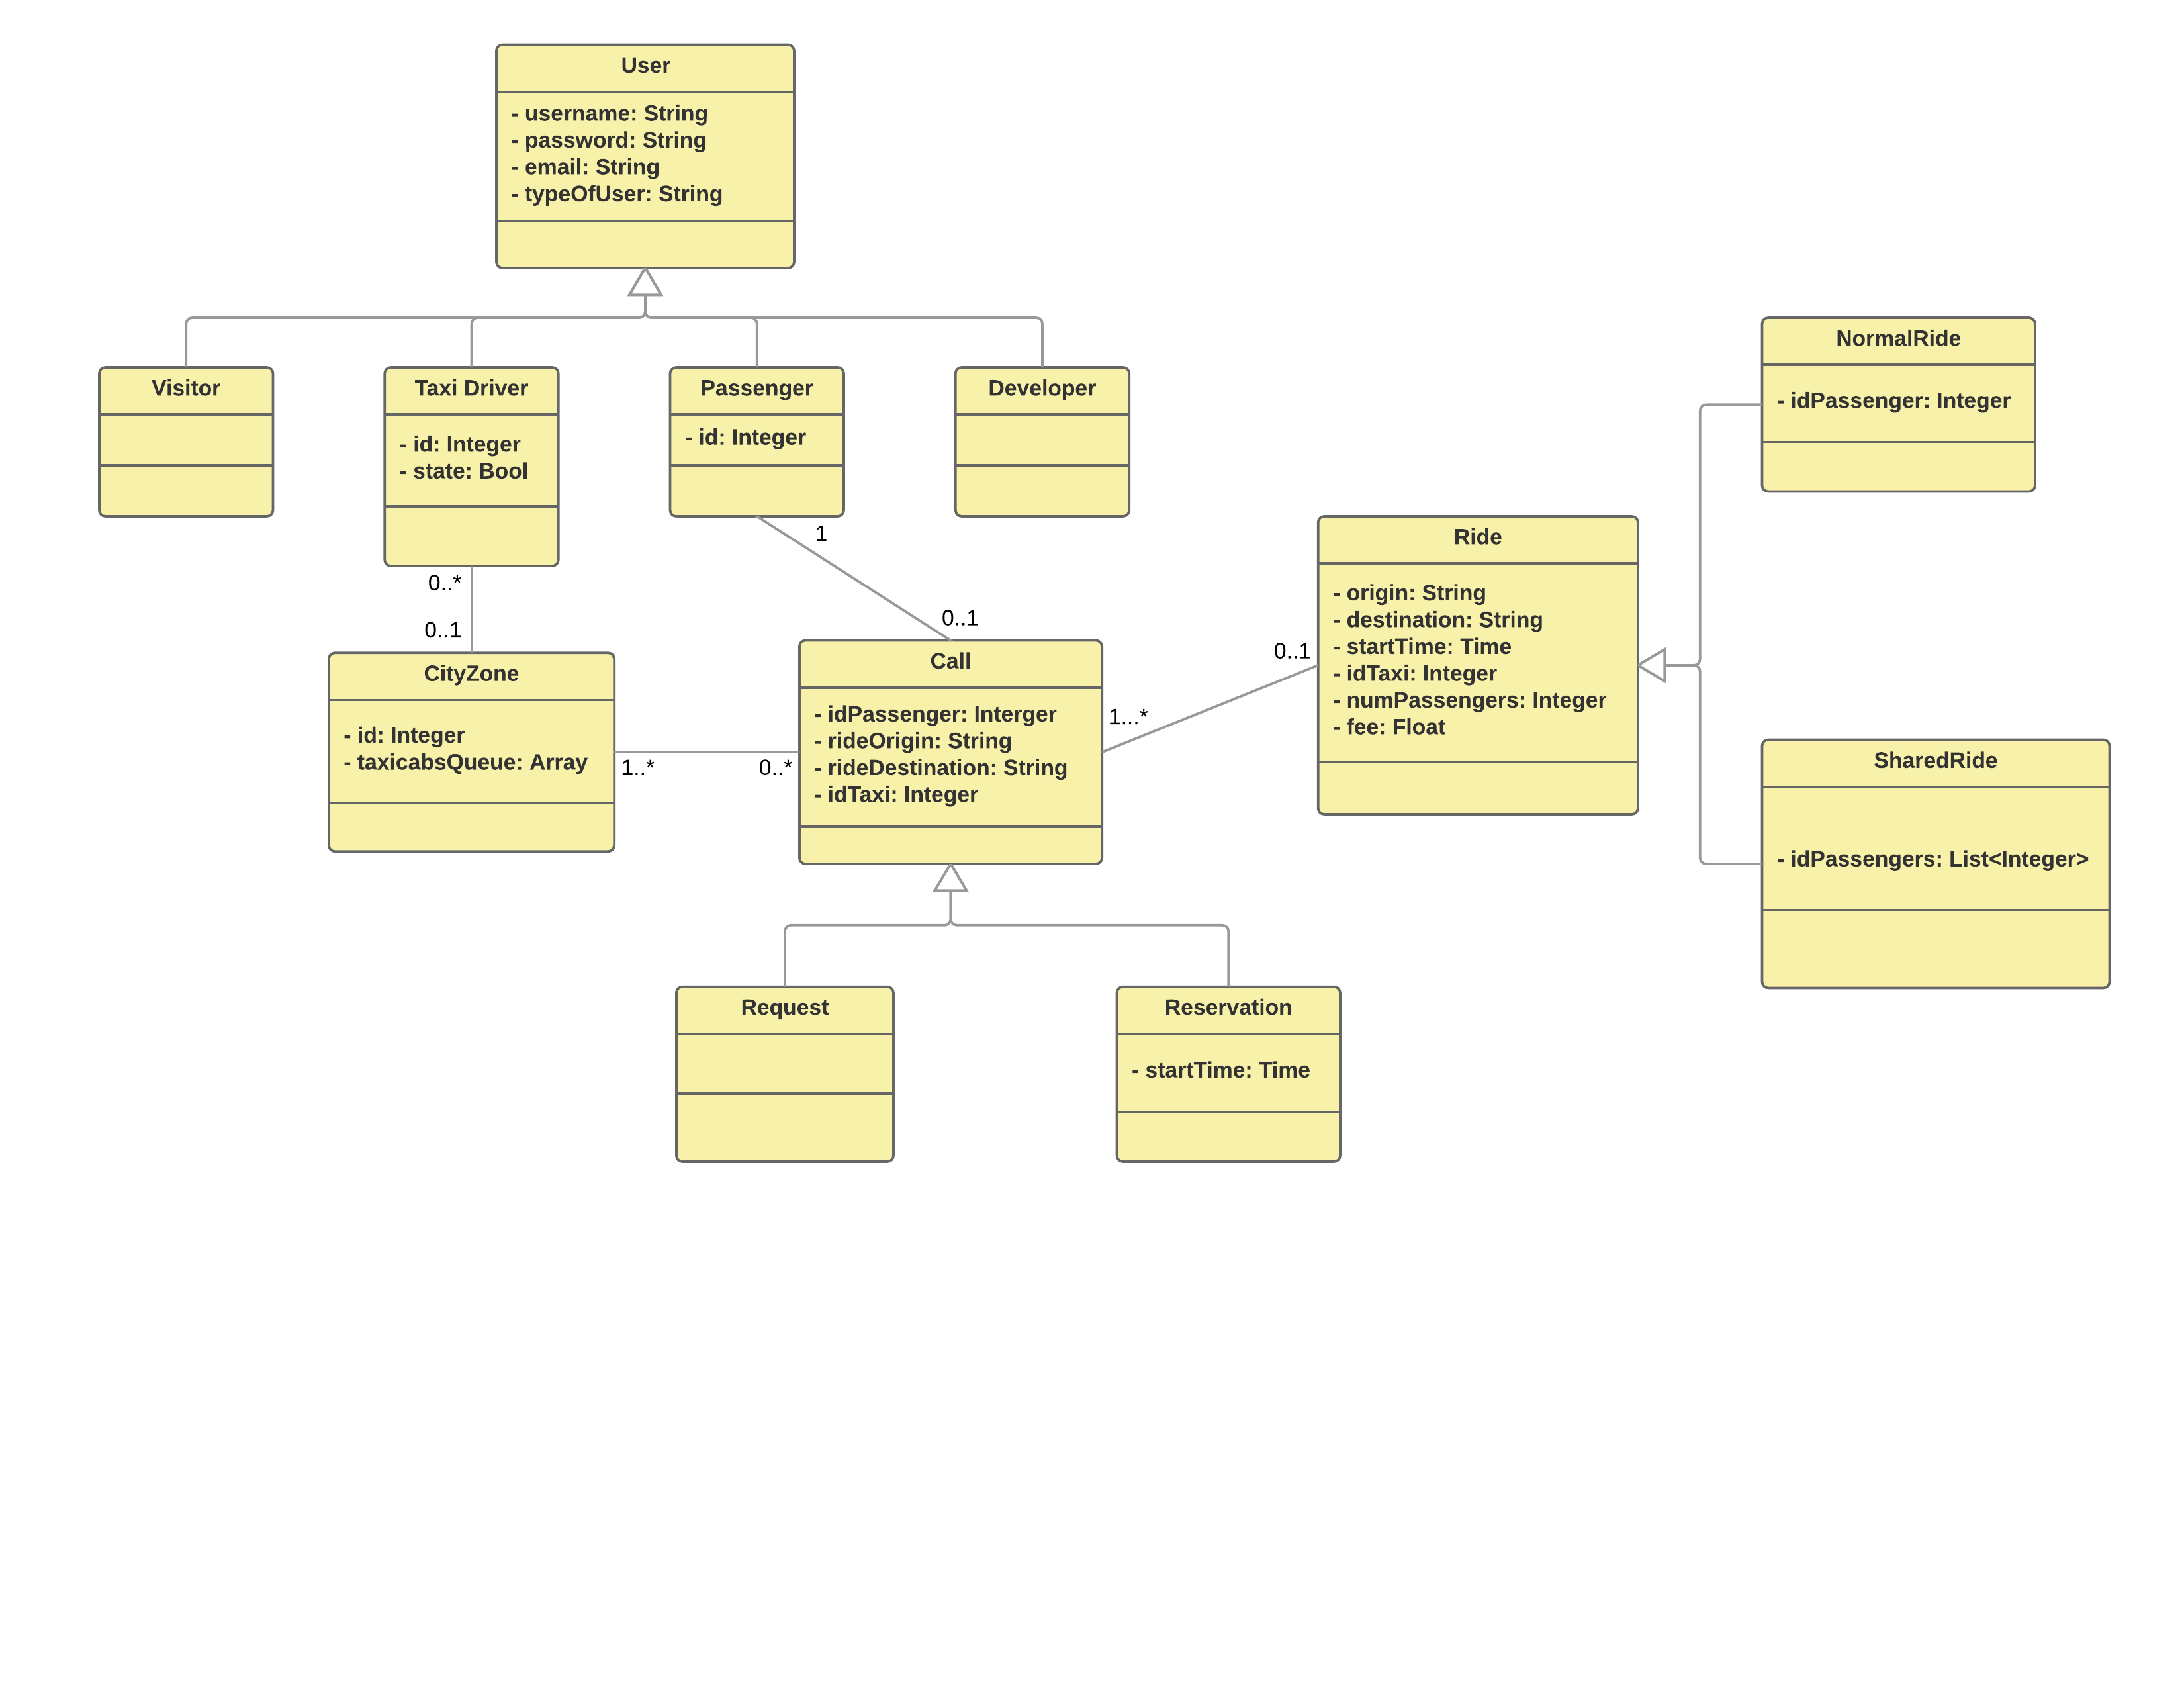
\includegraphics[width=\paperwidth]{cpt/img/ClassDiagram}
\caption{Class Diagram}
\label{fig:classdiag}
\end{figure}
\end{landscape}

\section{Sequence Diagrams}

\subsubsection{Log In}

\begin{figure}[htbp]
\centering
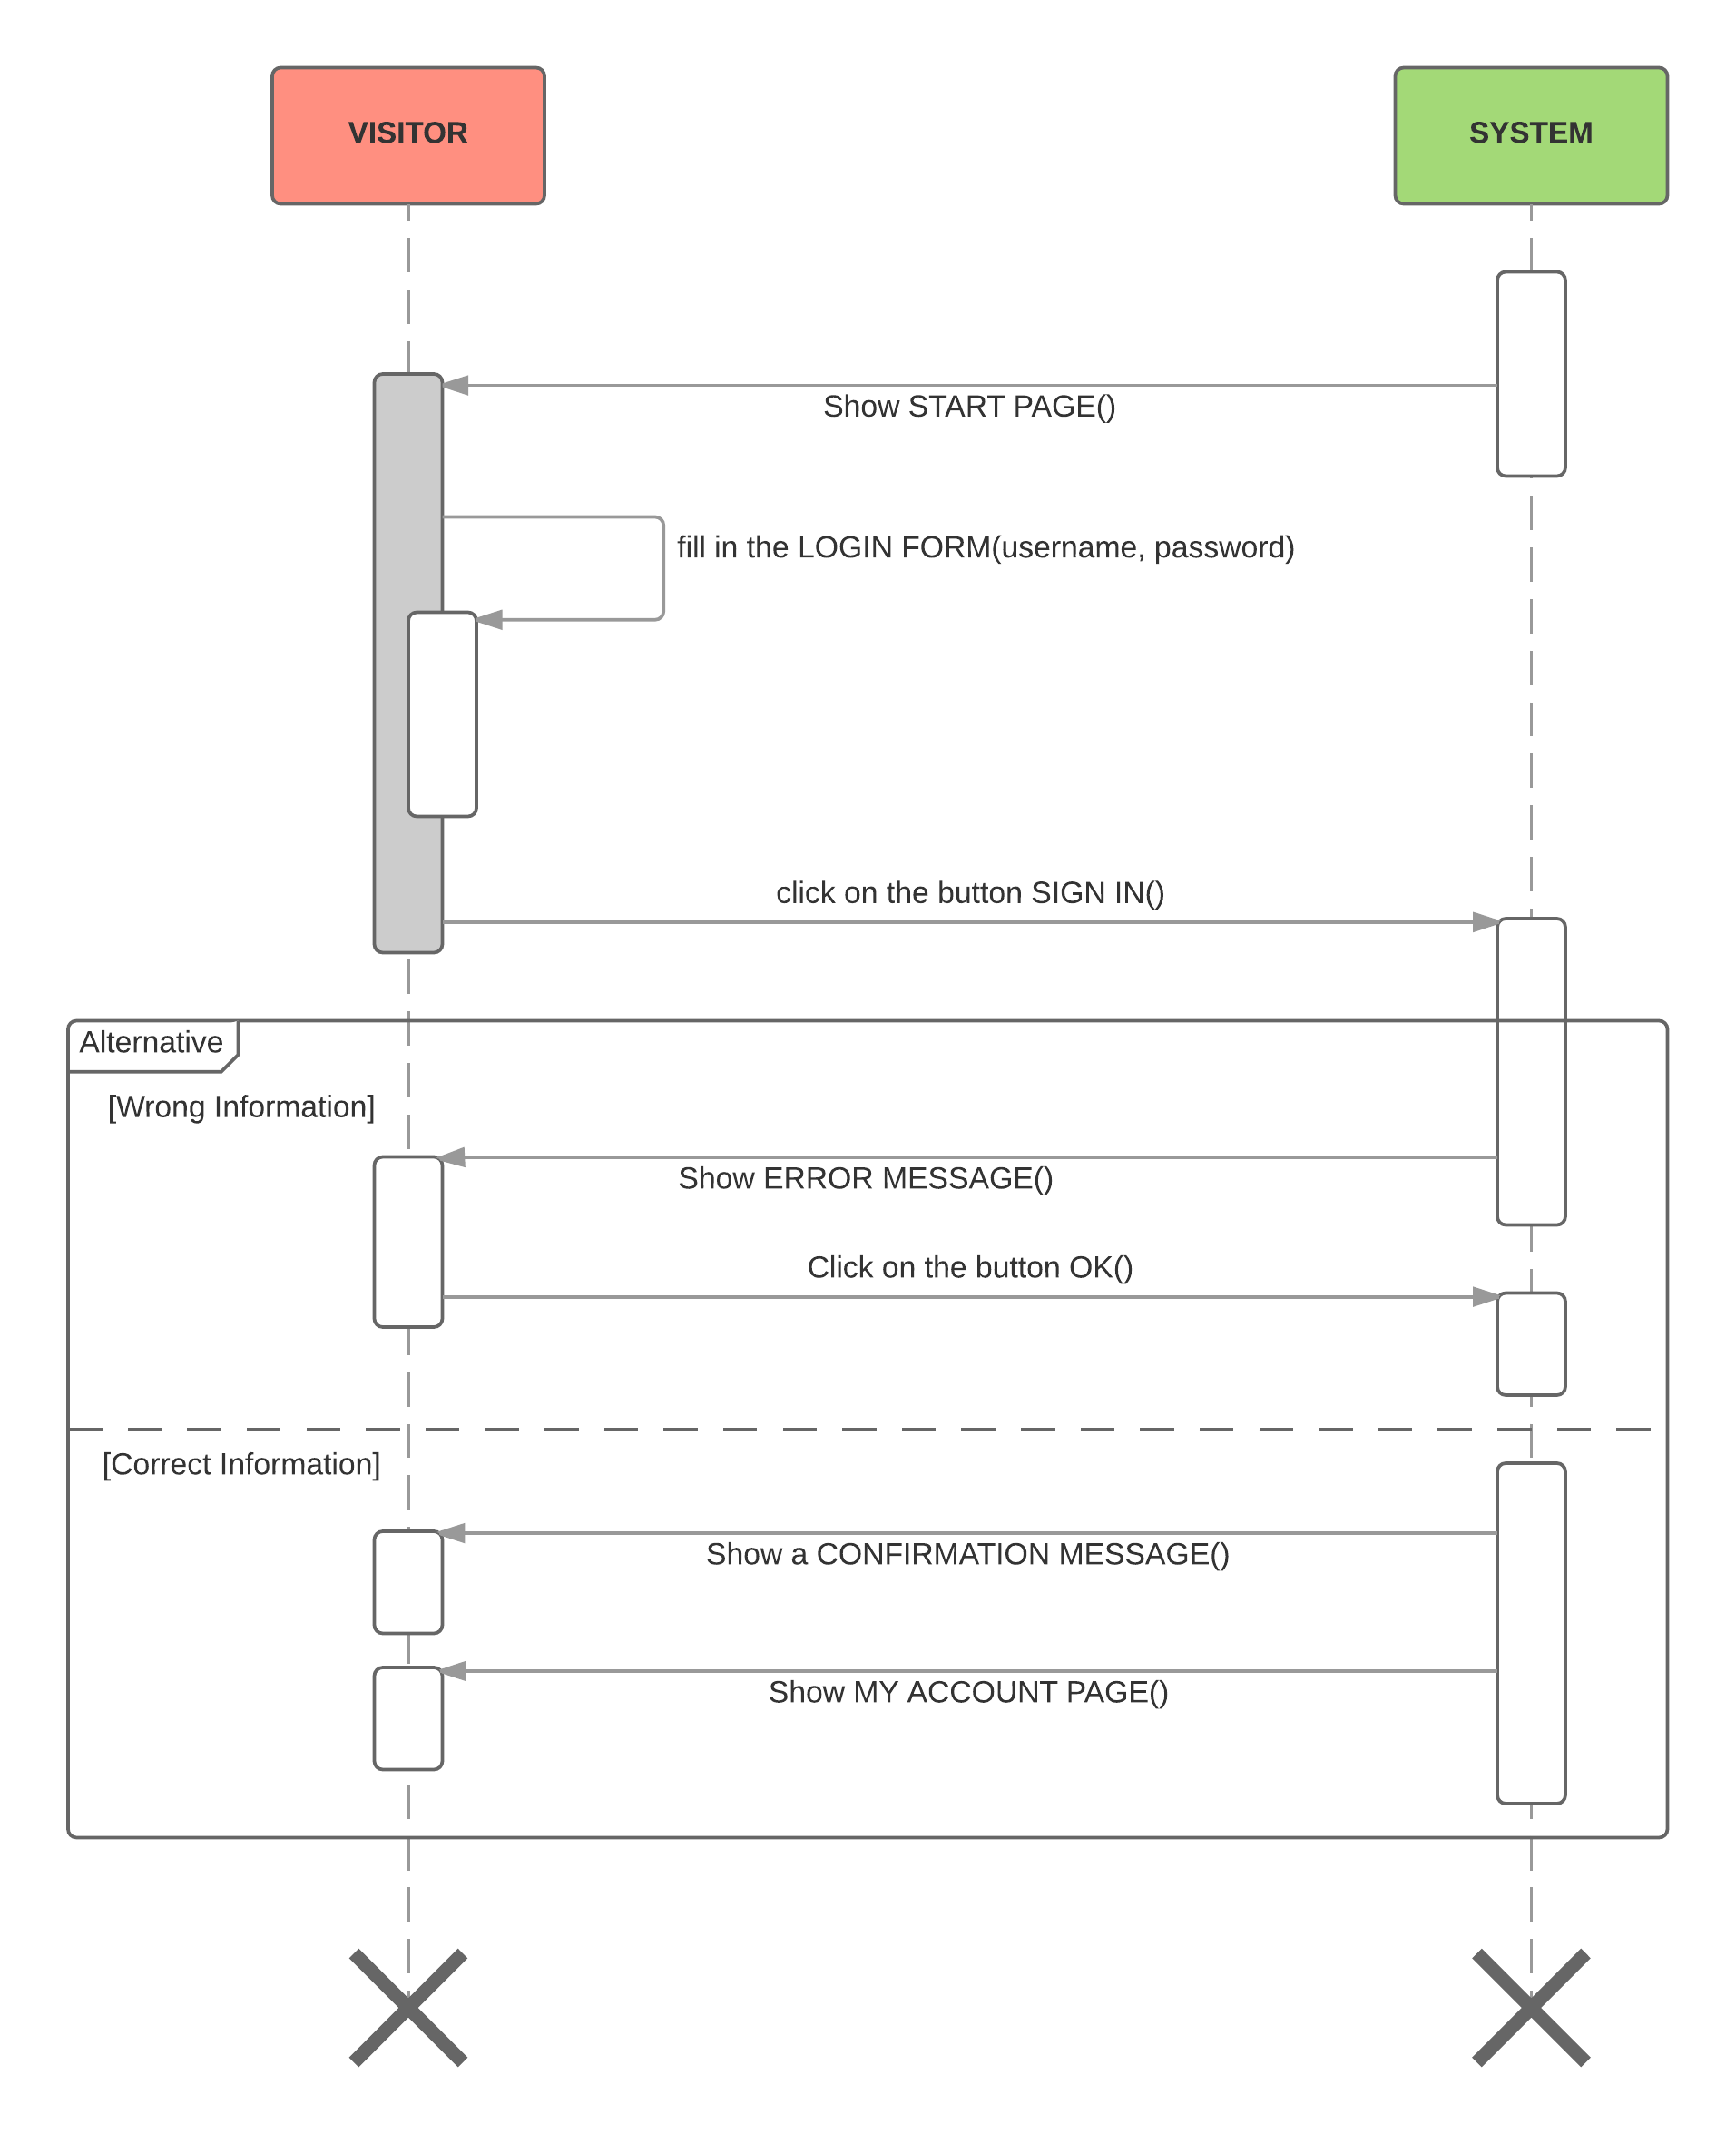
\includegraphics[width=0.9\textwidth]{cpt/img/SequenceLogin}
\caption{Sequence Diagram for Log In}
\end{figure}
\clearpage

\subsubsection{Request a Taxi Ride}

\begin{figure}[htbp]
\centering
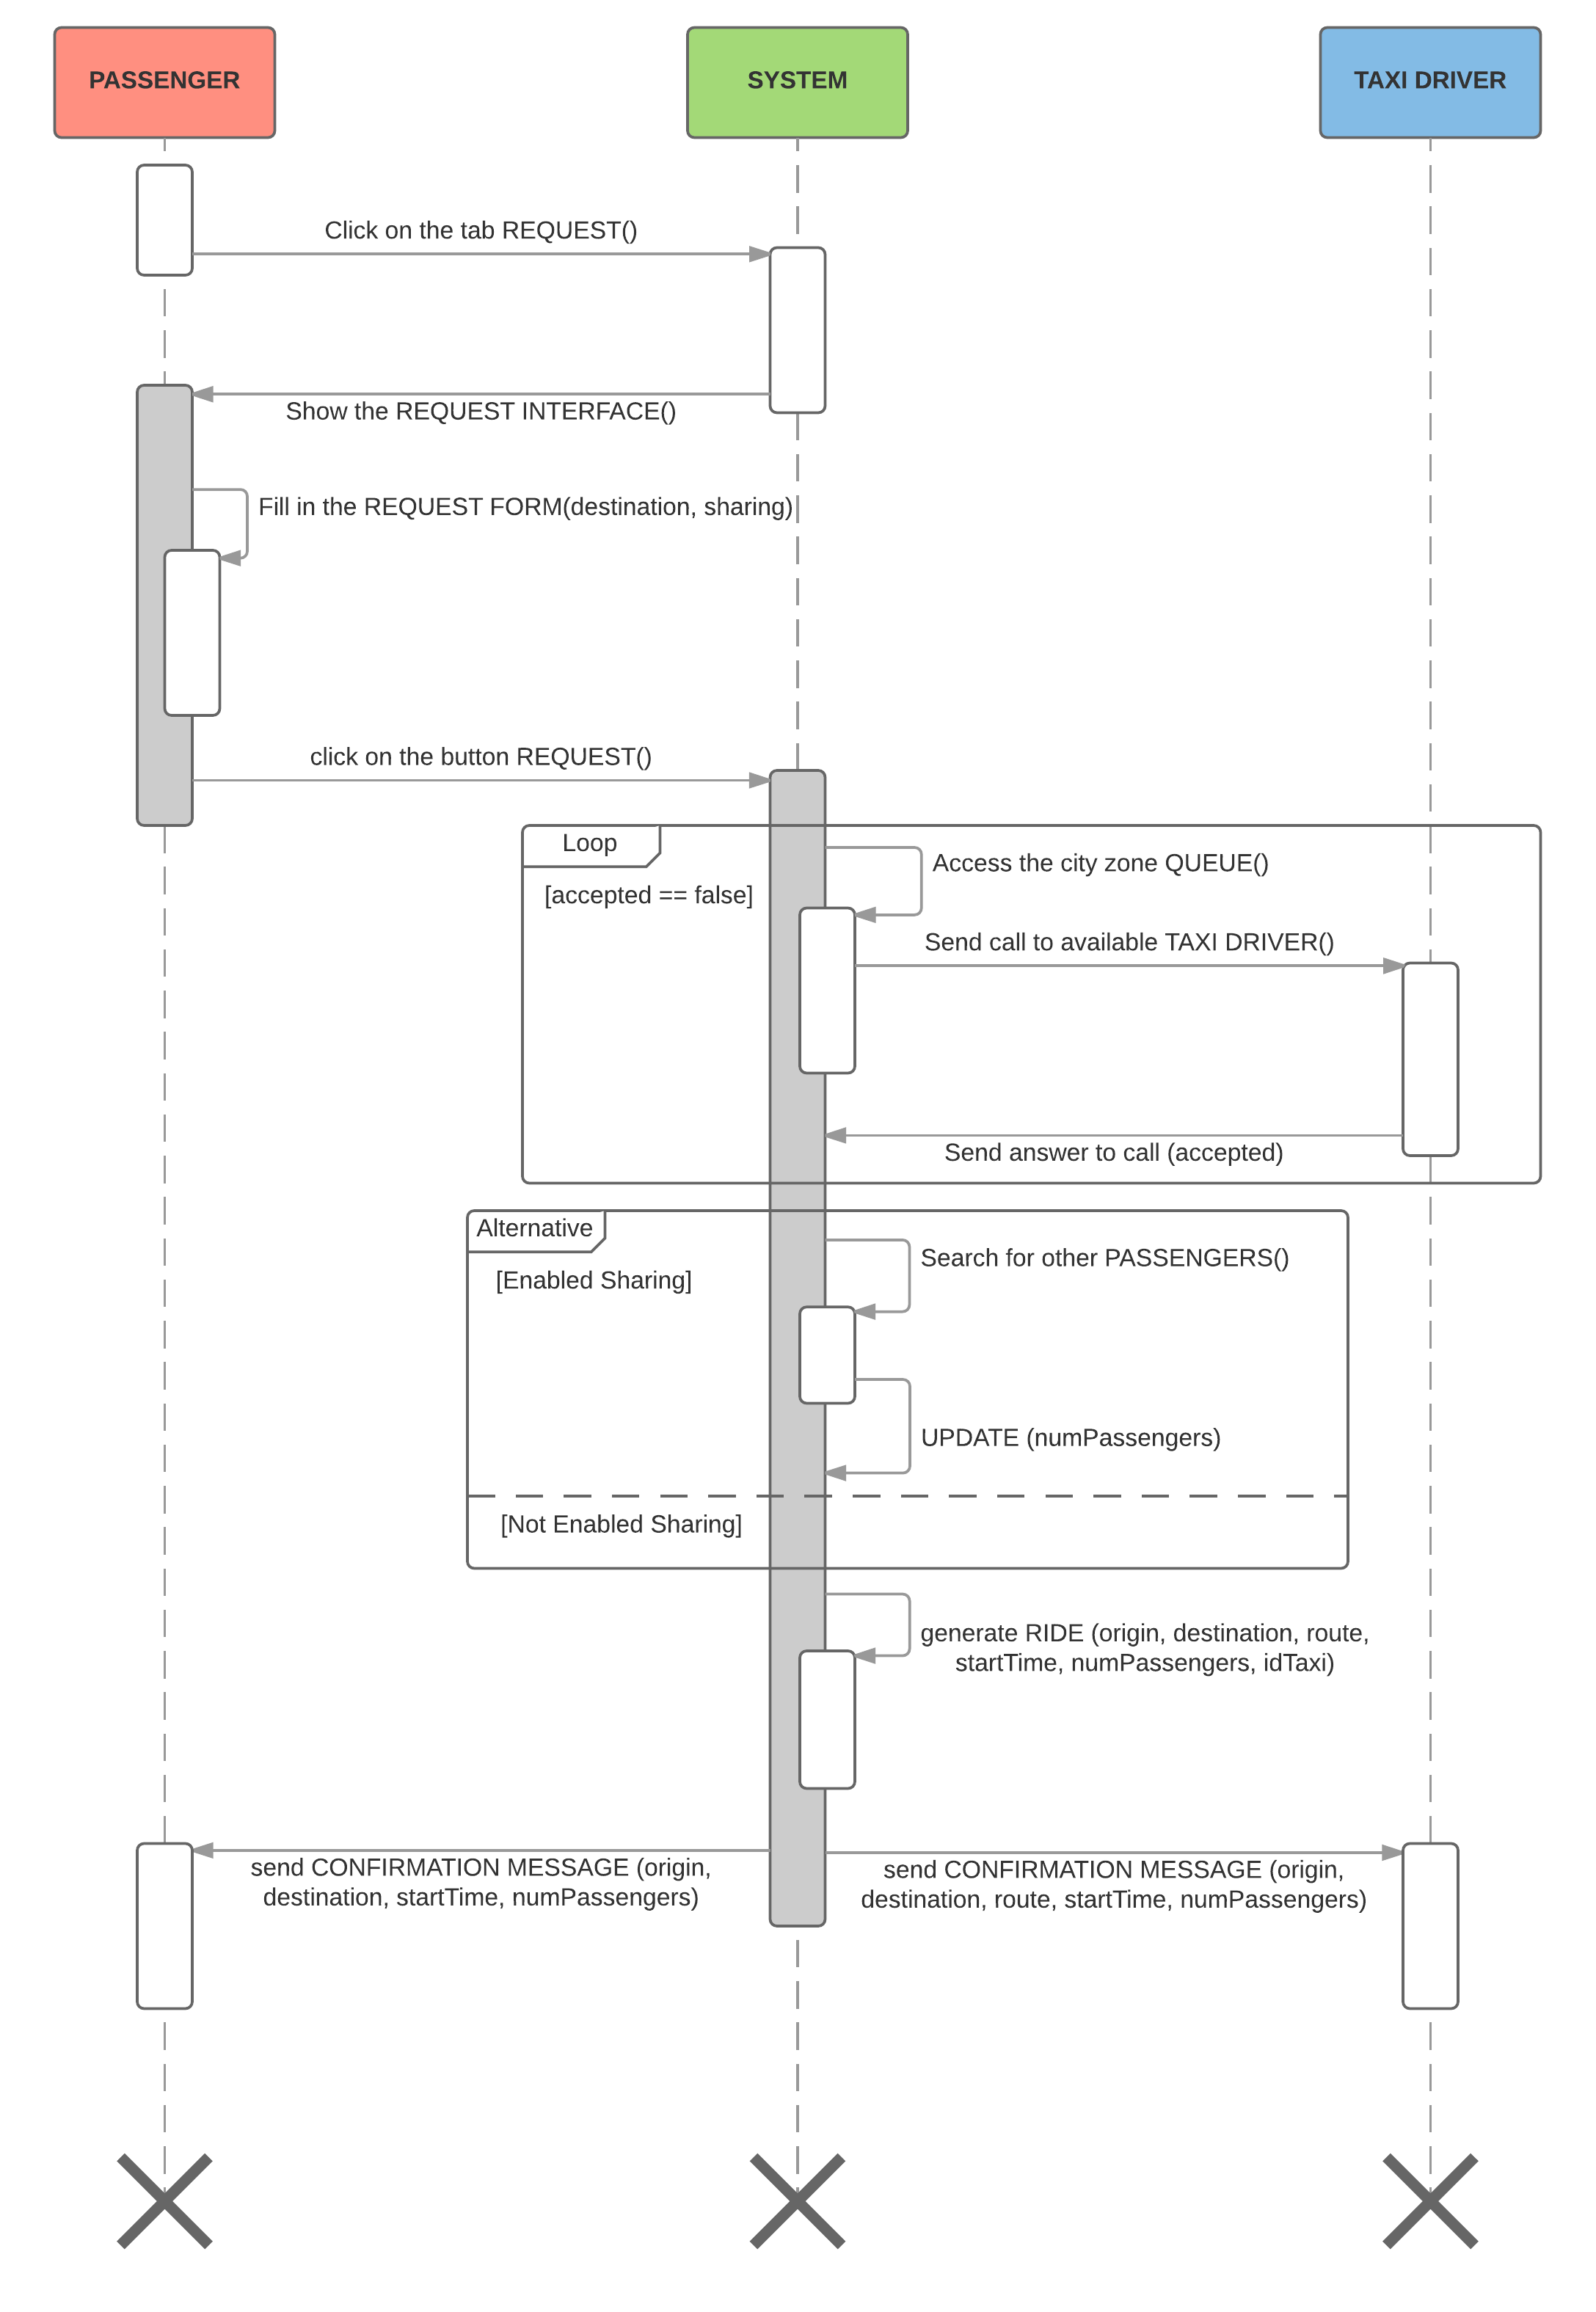
\includegraphics[width=0.8\textwidth]{cpt/img/SequenceRequest}
\caption{Sequence Diagram for Request a Taxi Ride }
\end{figure}
\clearpage

\subsubsection{Reserve a Taxi Ride}

\begin{figure}[htbp]
\centering
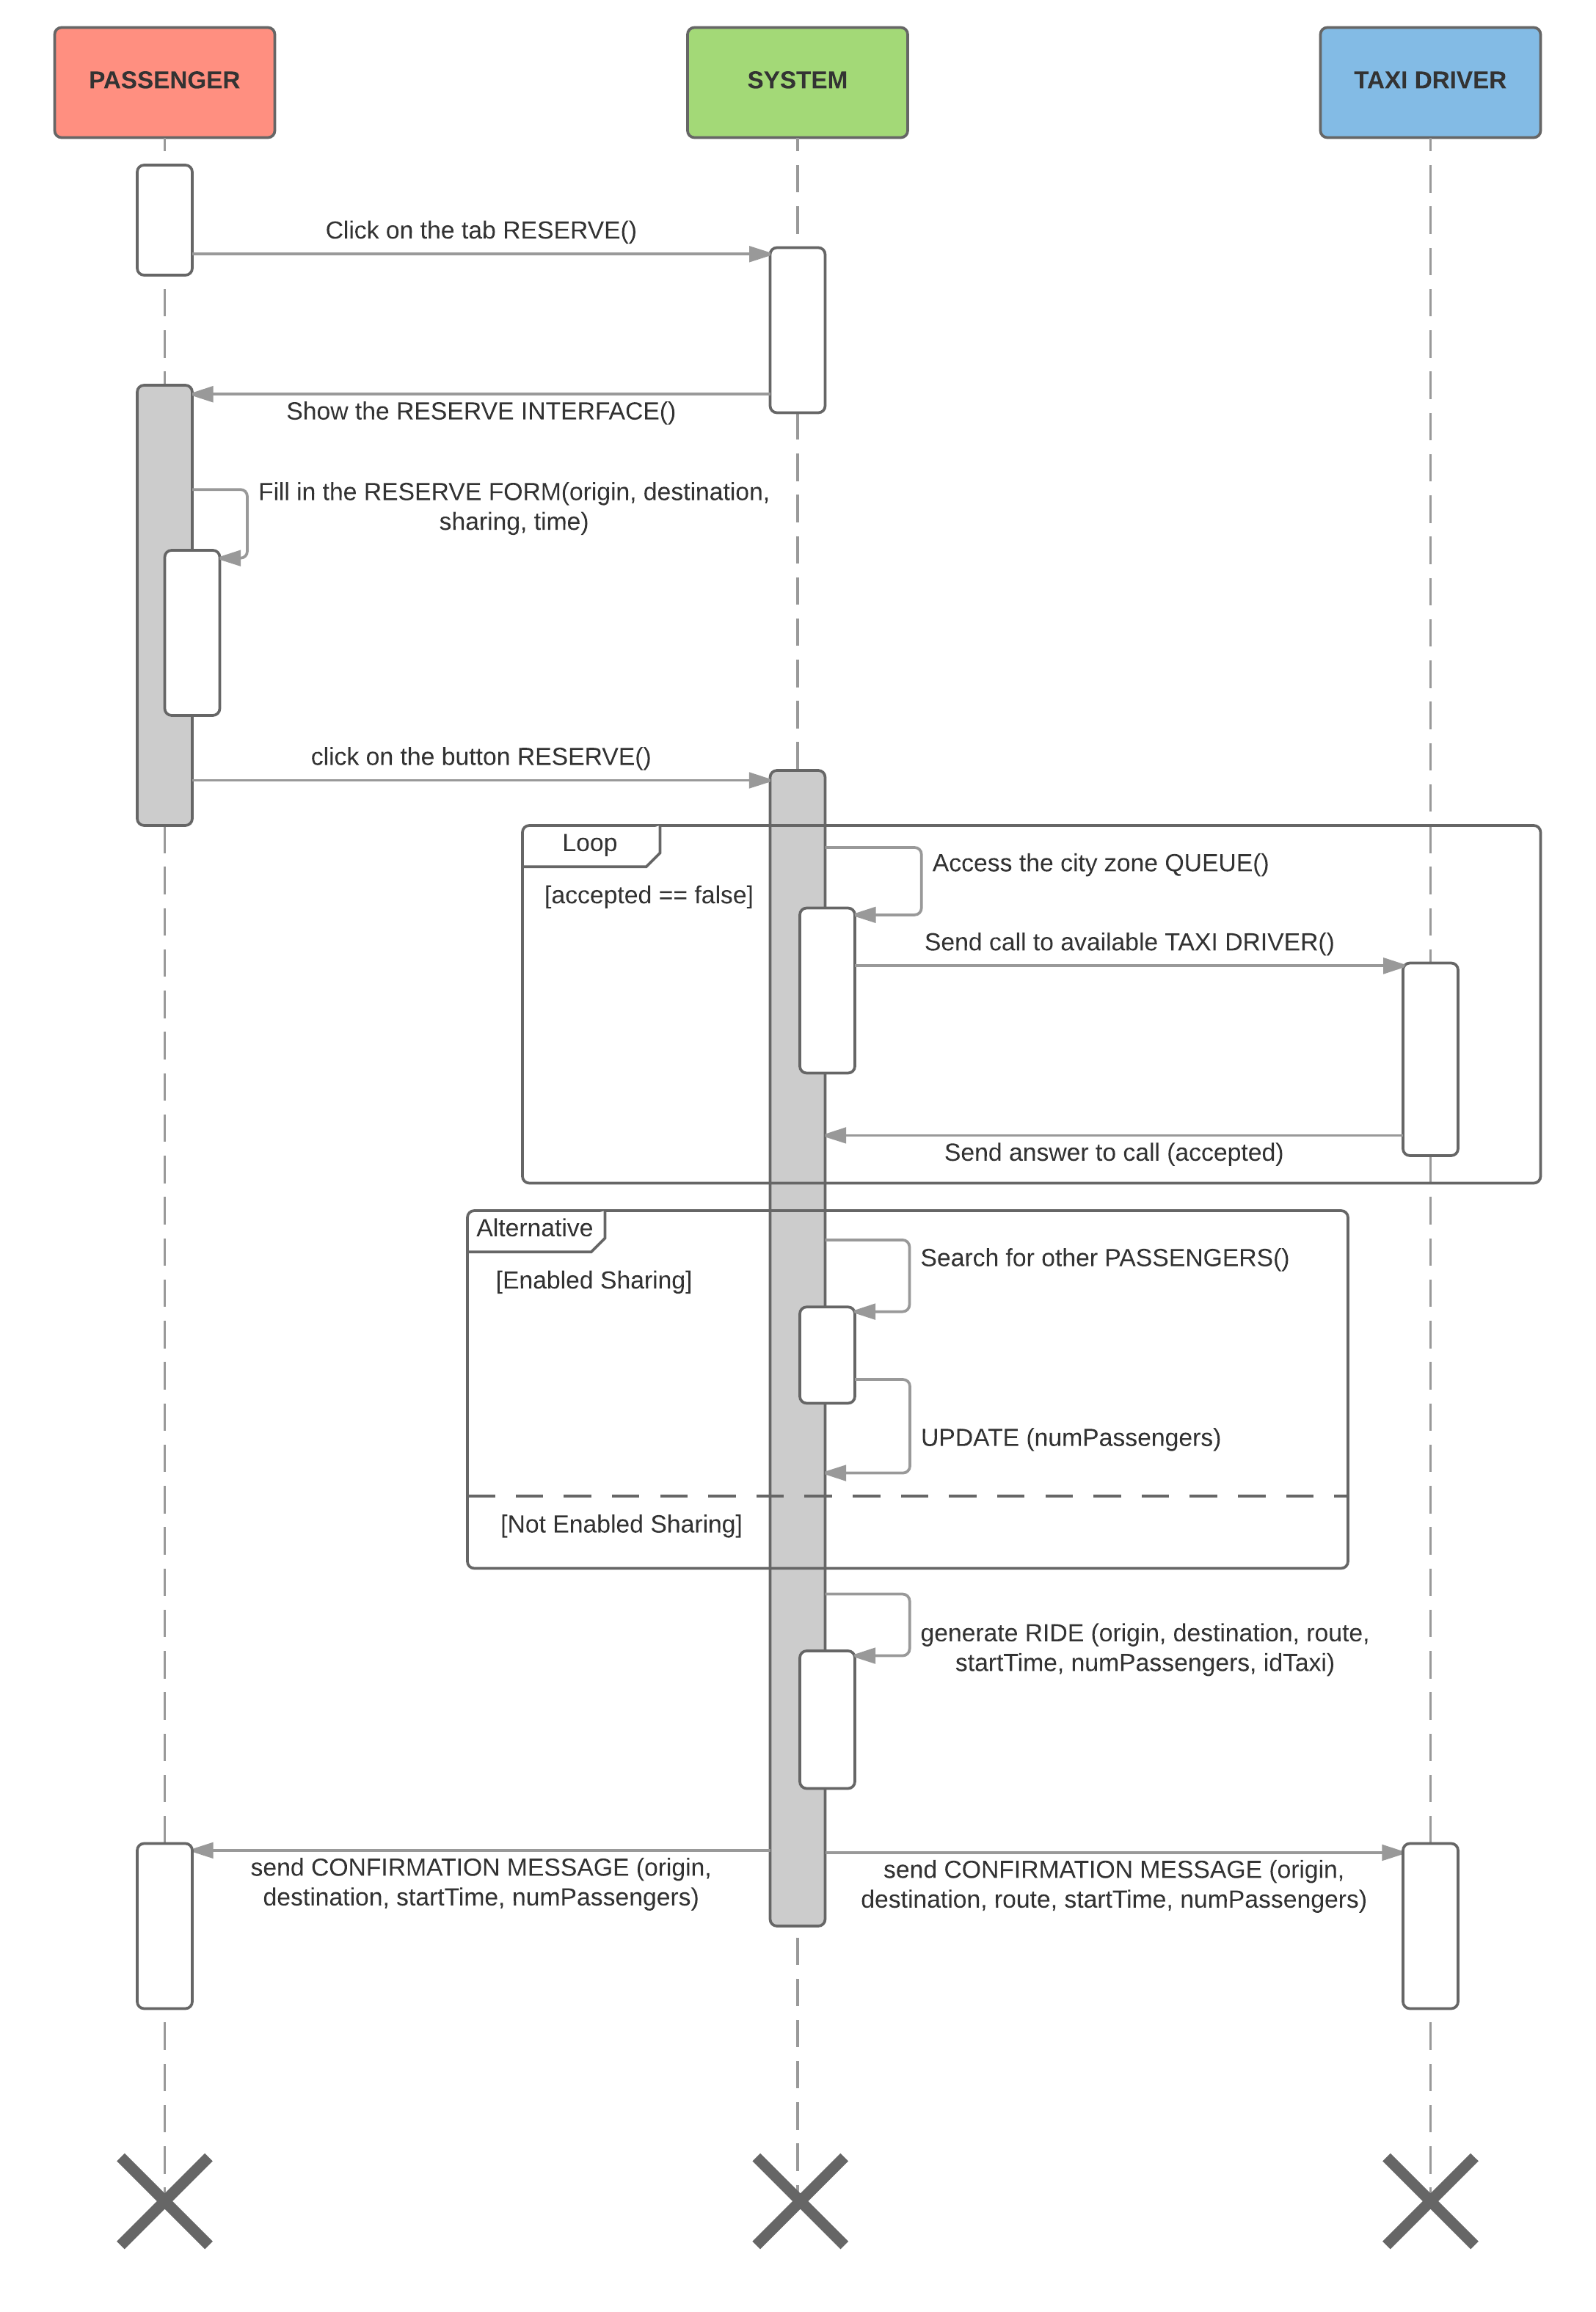
\includegraphics[width=0.8\textwidth]{cpt/img/SequenceReserve}
\caption{Sequence Diagram for Reserve a Taxi Ride}
\end{figure}
\clearpage

\subsubsection{Introduce Modifications in the System}

\begin{figure}[htbp]
\centering
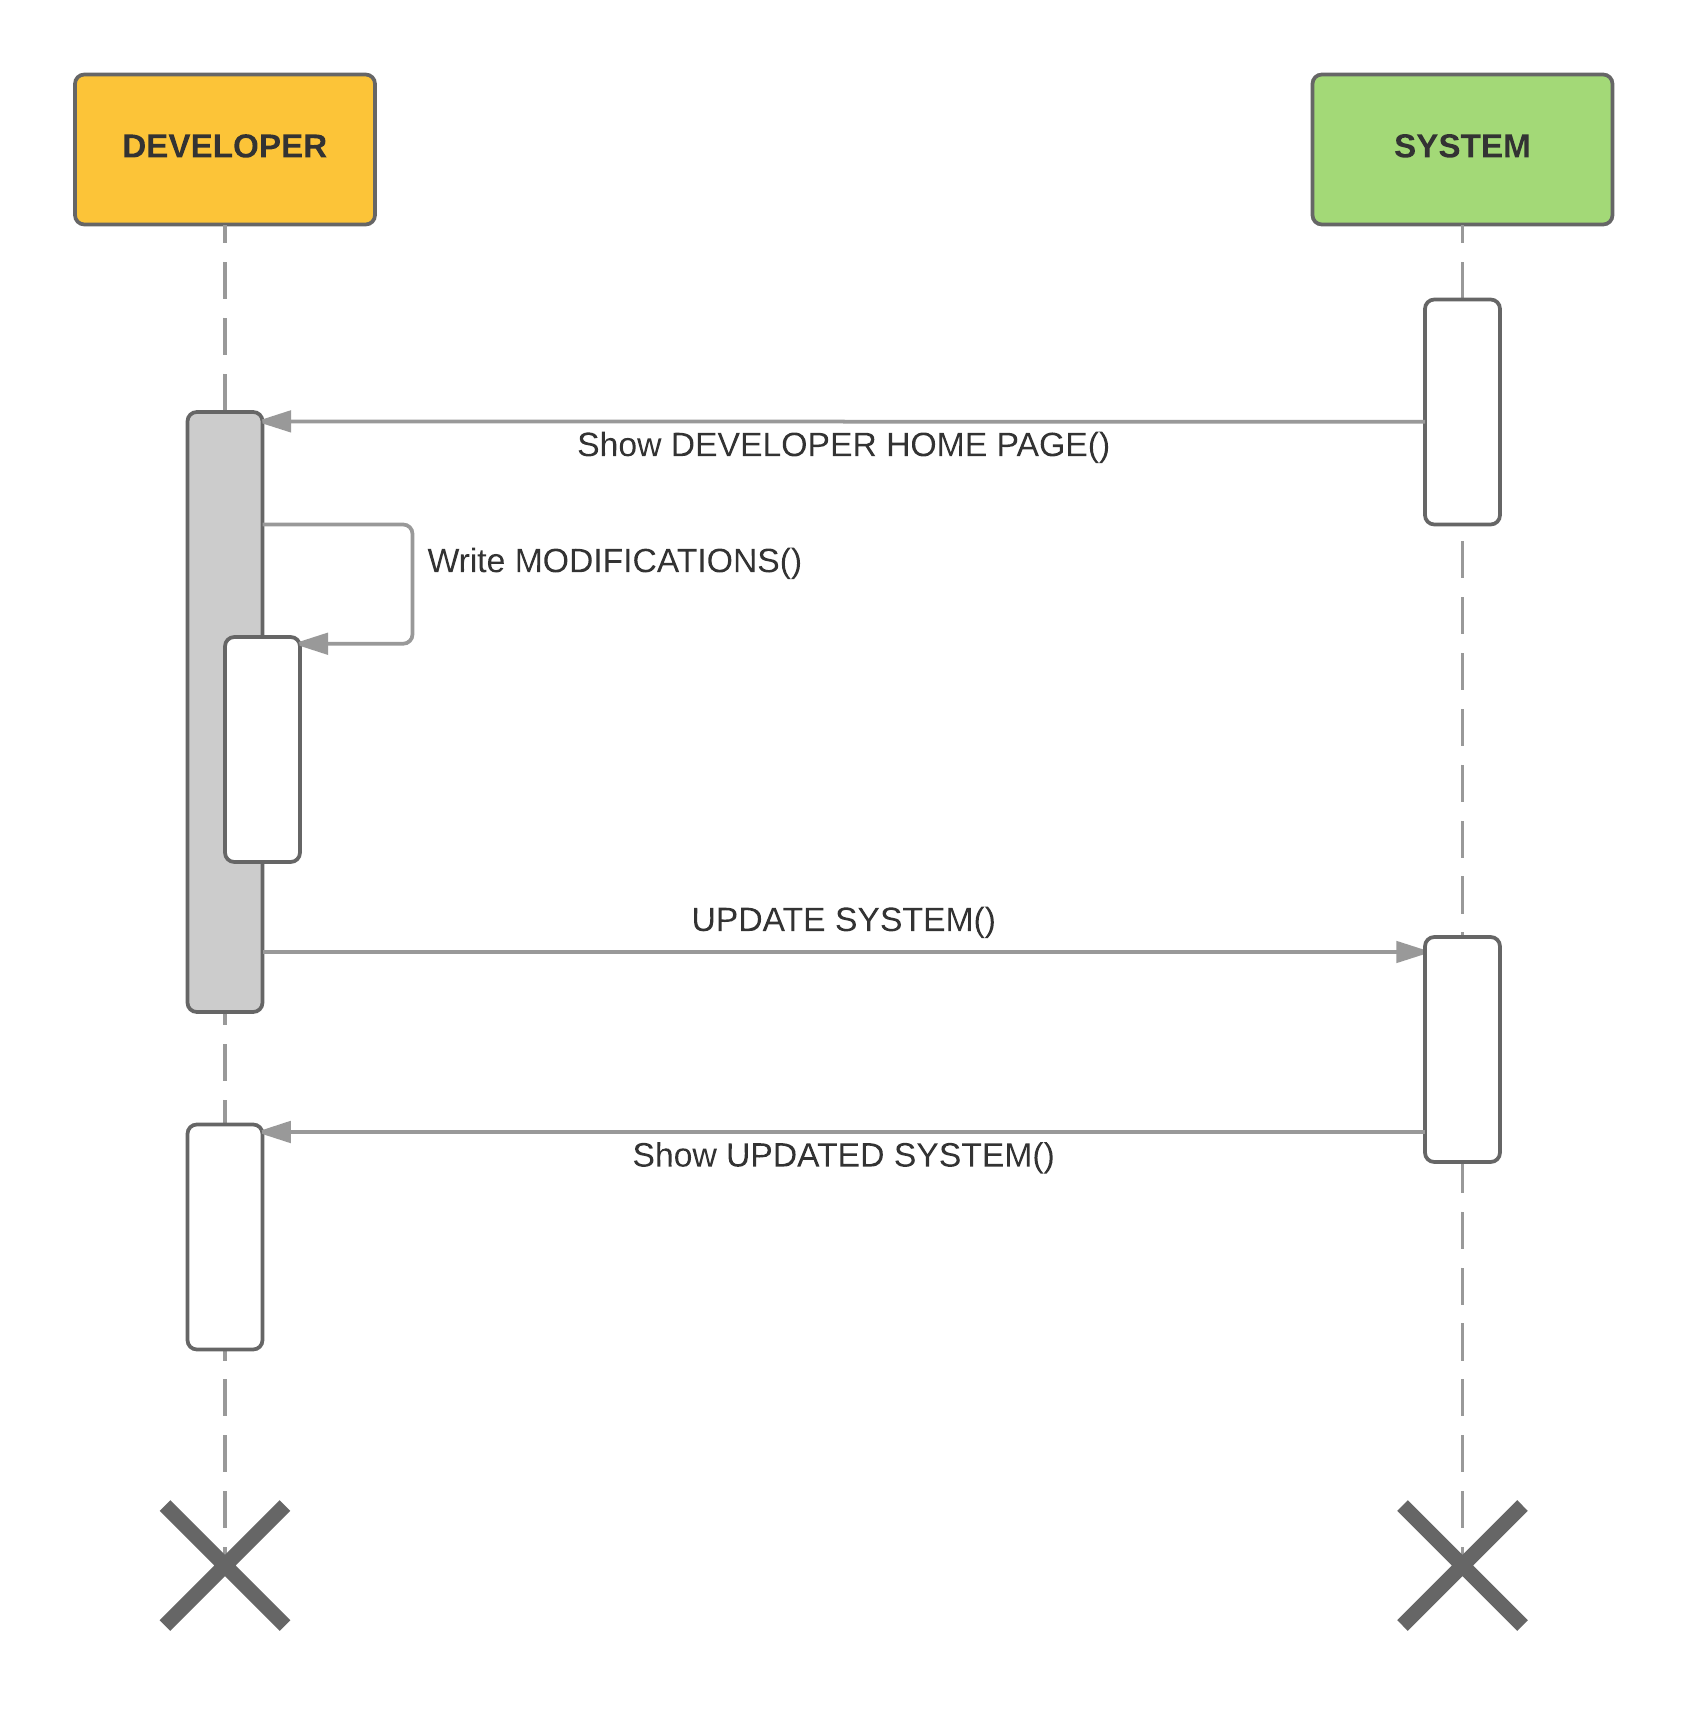
\includegraphics[width=\textwidth]{cpt/img/SequenceModify}
\caption{Sequence Diagram for Introducing Modifications}
\end{figure}
\clearpage

\section{State Chart Diagrams}
In this section the behavior of some entities presented in Figure \ref{fig:classdiag} is exposed using UML state chart diagrams. The following state chart diagrams will give a simplified vision of entire application:

\subsubsection{State Chart Diagram for Passengers}

\begin{figure}[htbp]
\centering
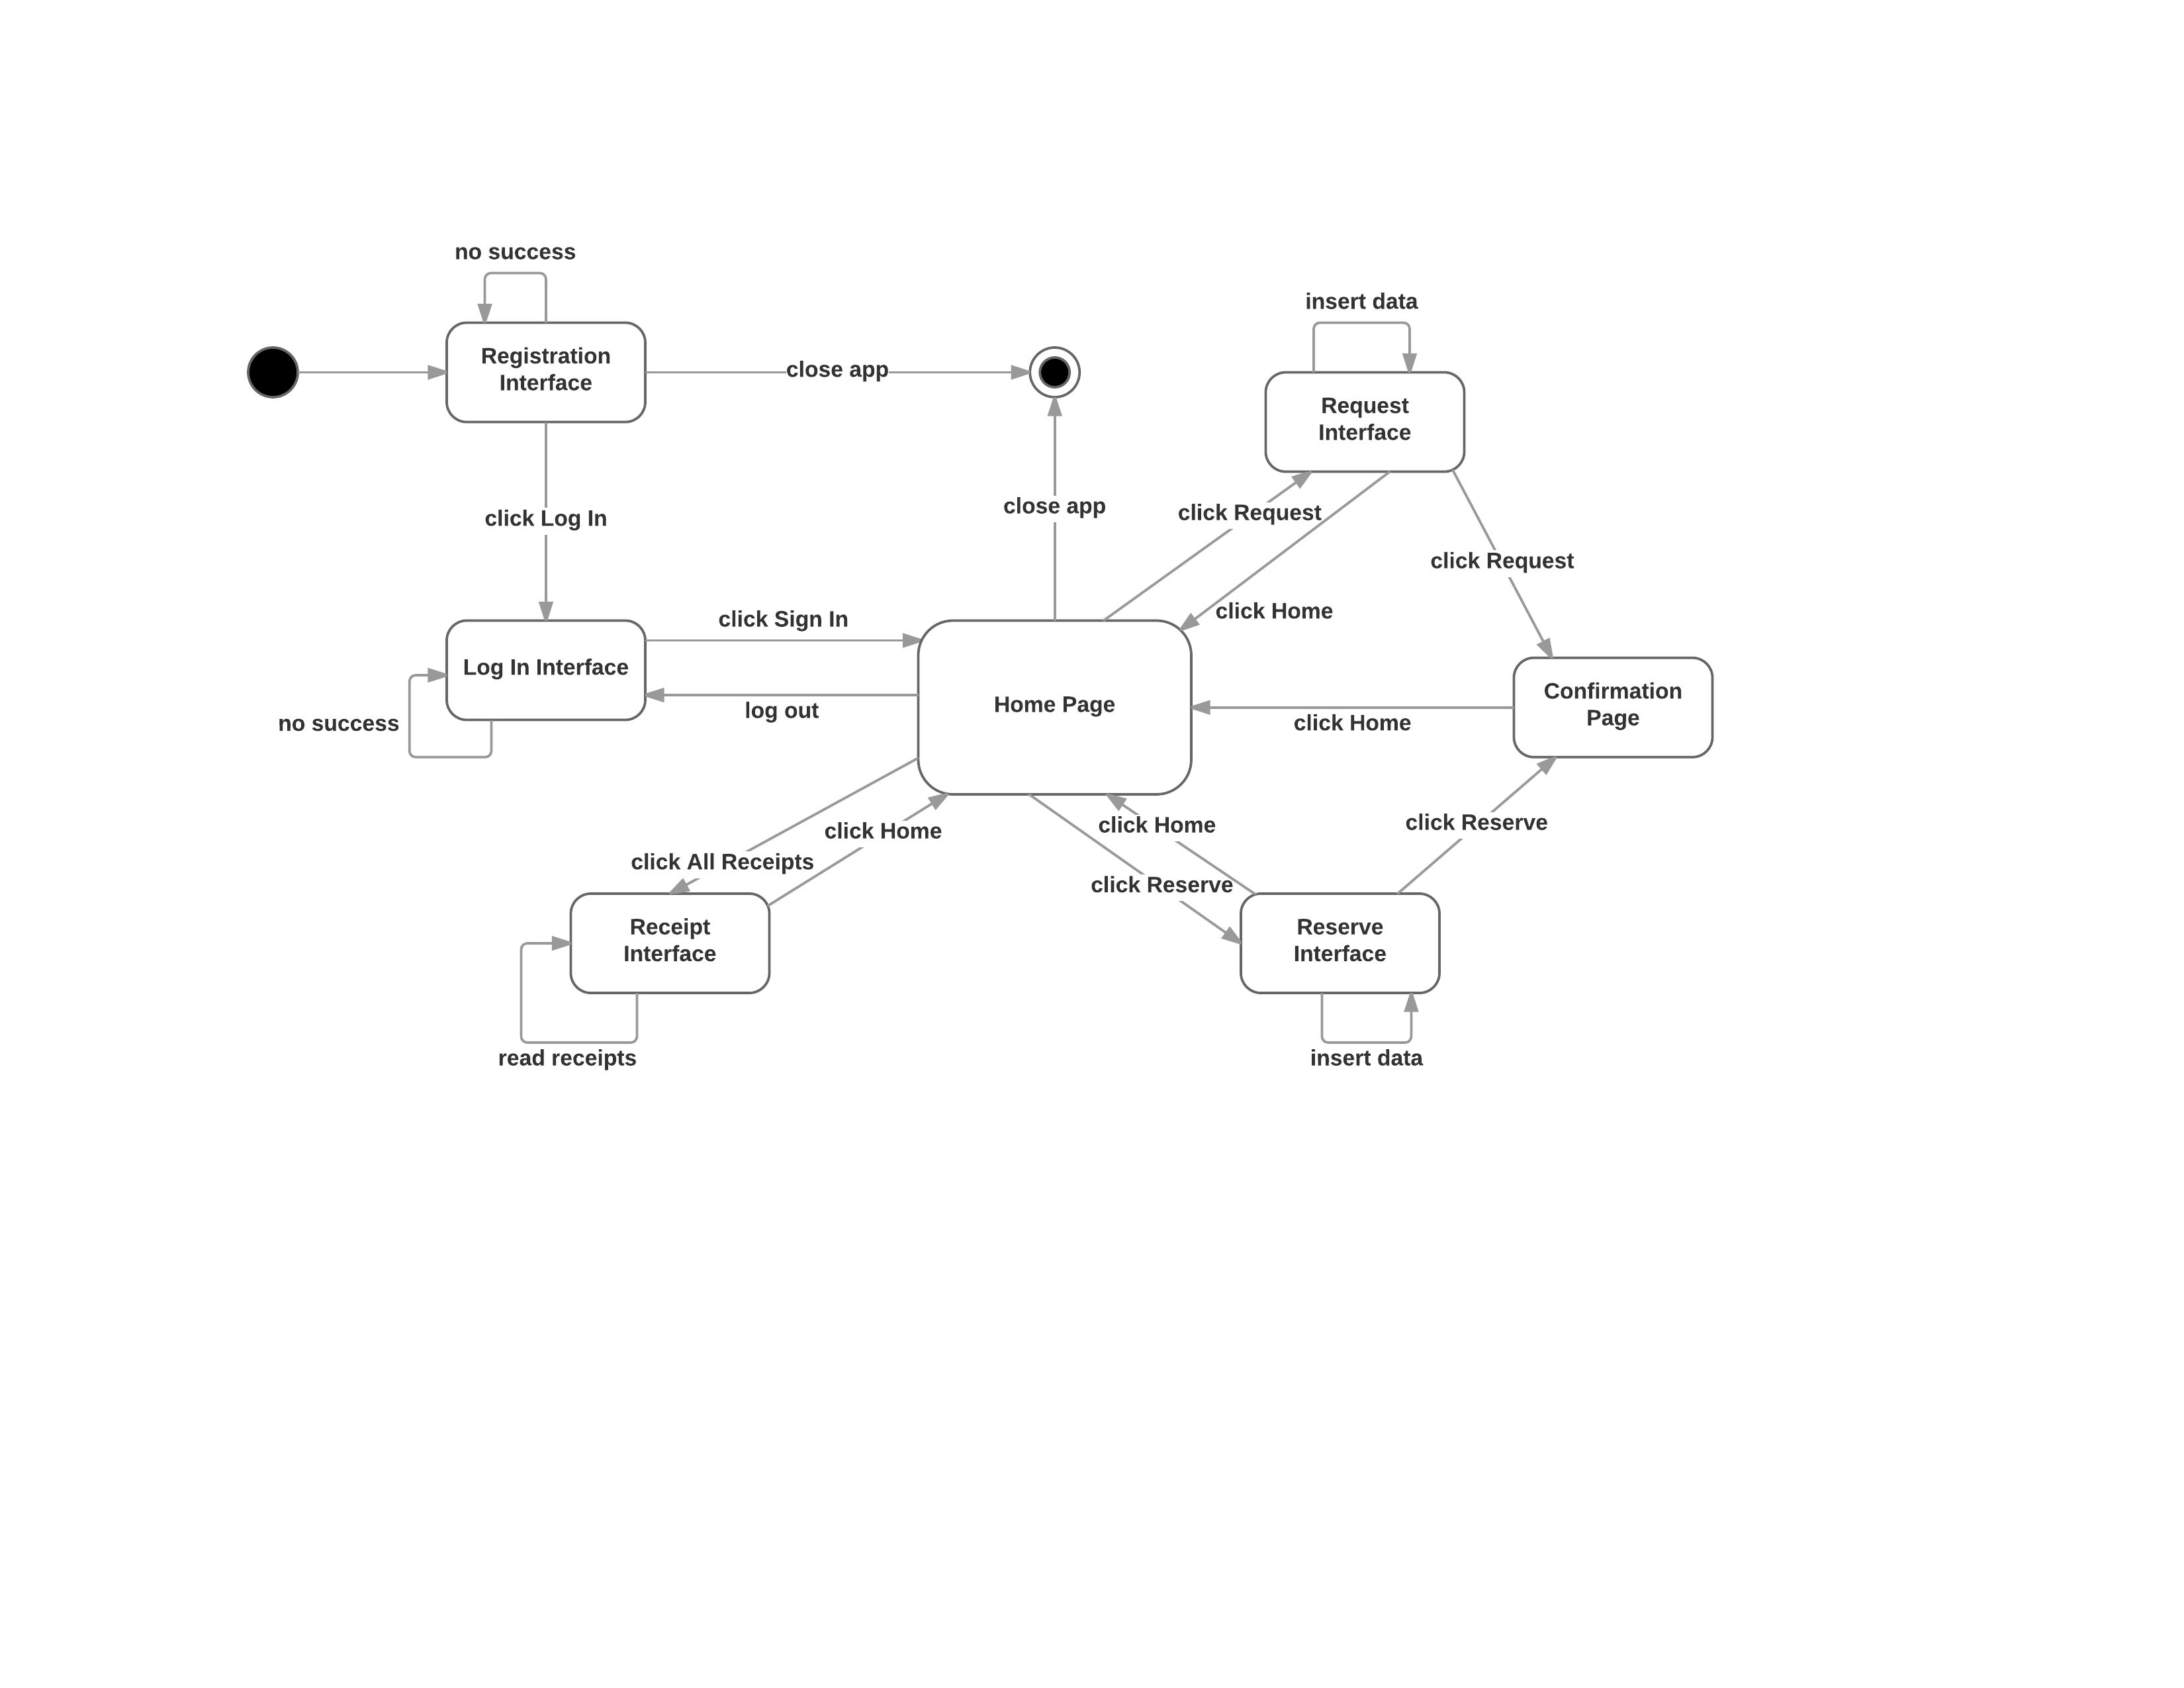
\includegraphics[width=\textwidth]{cpt/img/StateChartPass}
\caption{State Chart Diagram for Passengers}
\end{figure}
\clearpage

\subsubsection{State Chart Diagram for Taxi Drivers}

\begin{figure}[htbp]
\centering
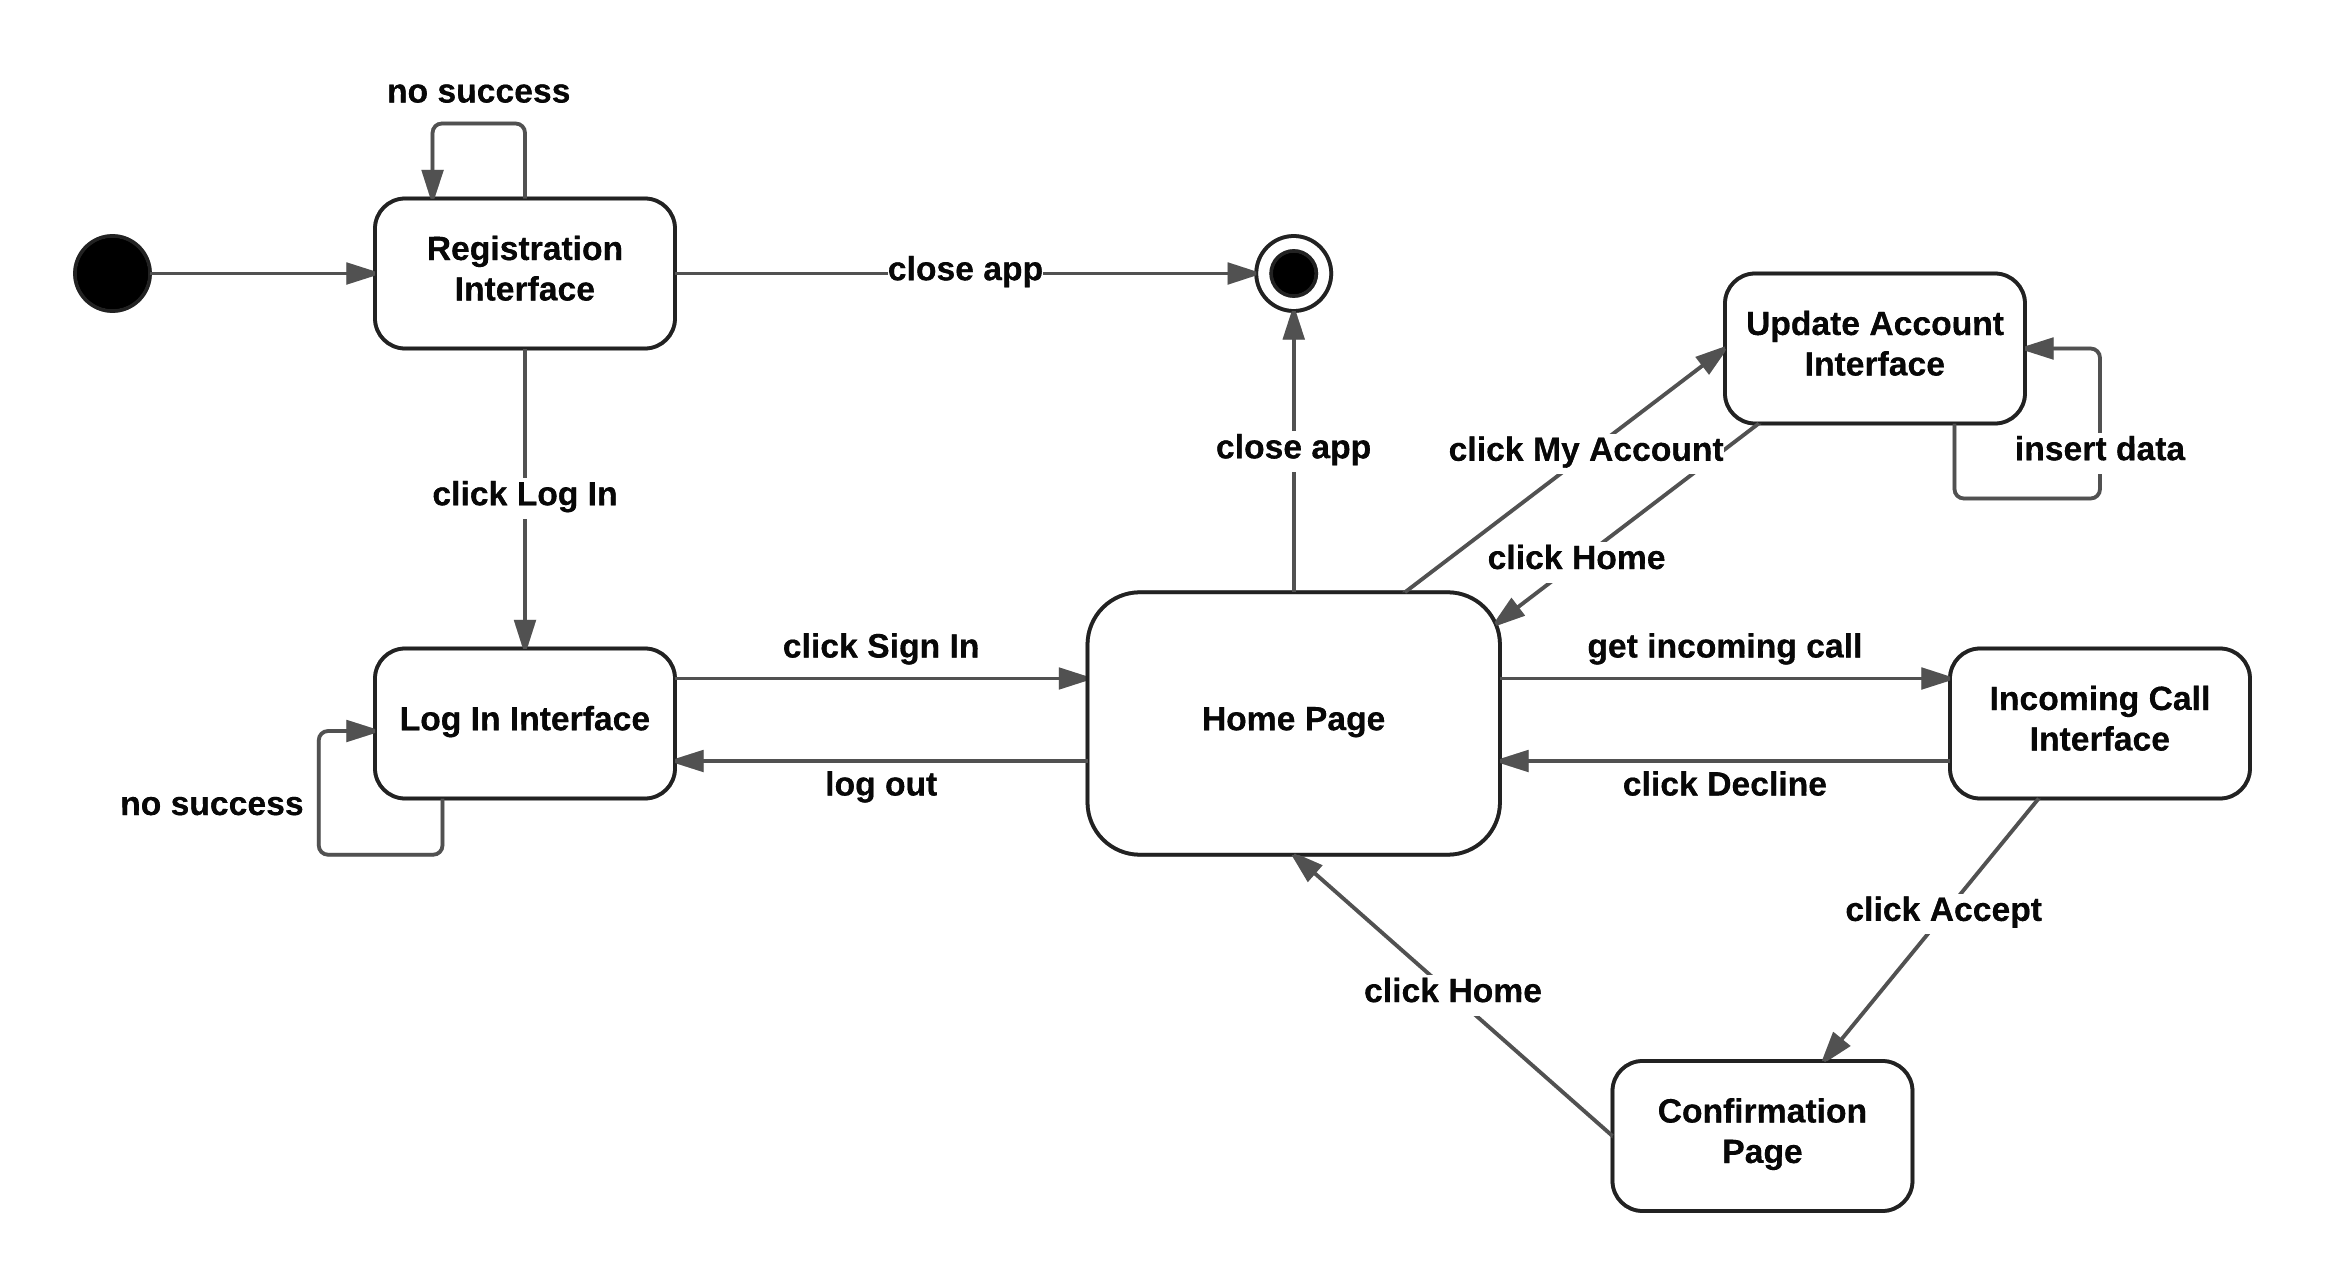
\includegraphics[width=\textwidth]{cpt/img/StateChartDriver}
\caption{State Chart Diagram for Taxi Drivers}
\end{figure}